\subsection{Thompson Sampling}

In this section we evaluate the gains produced by Thompson sampling (TS) in a high throughput virtual screening setting. For this, we perform experiments in which we sequentially sample molecules from an original library of candidate molecules. After each sampling step, we calculate the 1\% recall, that is, the fraction of the top 1\% of molecules from the original library that are found among the sampled ones. Each sampling step consists in selecting a batch of molecules among those that have not been sampled so far. In the Malaria and One-dose data sets we use bathes of size 200. These data sets contain each one around 20,000 molecules. By contrast, the CEP data set contains 2 million molecules. In this latter case, we use batches of size 1000.

We compare the performance of TS with that of 

Figure \ref{fig:thompson_1pc} that the Thompson sampling methodology significantly outperforms the Monte Carlo, and also offers increased performance and robustness than the greedy sampling methodology.  This is indicative of the importance of building in exploration into the sampling strategy, rather than relying on purely exploitative methods.  The set in which the greedy methodology performs best is the Clean Energy Project dataset - initially a greedy strategy yields a more enriched library of molecules, before eventually being overtaken by the Thompson sampling after molecules contained within the initially discovered area are exhausted.  It is helpful in cases such as this to think of the early difference in performance between the greedy and the Thompson strategies as a cost for building in exploration, which is eventually paid back when the 'prime' area of chemical space initially discovered by the greedy algorithm is exhausted.  It is, of course, possible to construct an example where all the molecules of interest are in one area of chemical space, and thus any time spent exploring other areas of chemical space is wasted.  In this regard, we point out that it is virtually impossible to construct an accurate information landscape without having all the information already collected, and that even with strongly localized libraries - such as the Clean Energy Project - a greedy strategy is quickly surpassed by Thompson sampling. 
  
\begin{figure}[htb]
\begin{center}
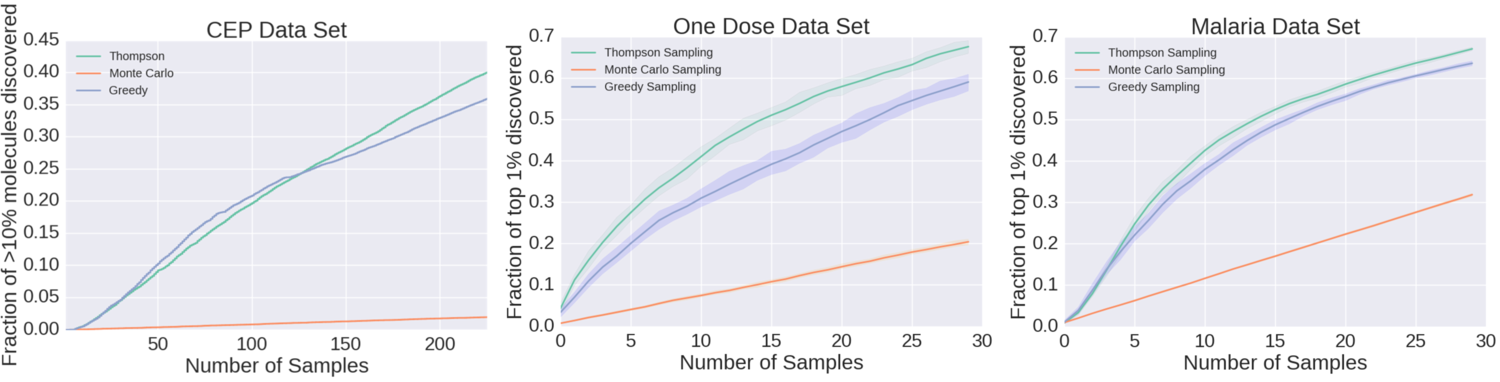
\includegraphics[width=0.8\columnwidth]{figures/thompson_tile/thompson_tile3.png}
\label{fig:thompson_1pc}
\caption{The recall of the Thompson sampling methodology for each of the datasets included in this study.  For the CEP dataset, the recall for molecules with a PCE $>10\%$ is reported, whilst for the One-Dose and Malaria datasets the recall for the top 1\% of targets is reported.  In addition to the baseline Monte Carlo sampling, we also include a greedy sampling approach, in which there is no exploration, but the training set is selected by exploiting the predictive power of the model.  The general lower performance of this model indicates the importance of balancing exploration and exploitation when choosing molecules for high-throughput virtual screening.}
\end{center}
\end{figure}
This effect can be seen more clearly in Figure \ref{fig:cep_lib}.  The greedy strategy (green) initially performs exceptionally well, with a significant enrichment over both Monte Carlo and Thompson sampling strategies.  This advantage quickly decays, however, as the Thompson sampling benefits from the exploration performed, and the derived improved description of potential desirable areas of chemical space. We emphasize that even the Clean Energy Project, with its strongly localized cluster of desirable molecules, demonstrates deficiencies in the greedy sampling strategy.  Indeed, some of the strength shown by the greedy sampling strategy can be attributed to the sheer size of the dataset, with respect to the others investigated within this study.  It is logical that a method whose strength lies in exploiting localized knowledge of an area of chemical space in which desirable molecules have been found will benefit from a dataset which contains a large number of molecules, and which has been designed combinatorially. It should also be noted that the success of a greedy methodology is also dependent on the existence of a wide-necked funnel in the information landscape - if a cluster of desirable molecules in chemical space is too tight, it is unlikely to be sampled in the initialization of the method.  Thus, it is unlikely to be discovered - at least in an `intelligent' manner - by a greedy sampling methodology; a situation which is strongly undesirable when building libraries for which each point is expensive to discover the ground truth value.
  
In order to put the importance of these results into context, we consider the saving in calculation time for the Clean Energy Project dataset. Thompson sampling, displays $>30x$ faster discovery than the Monte Carlo search, which is in itself faster than the exhaustive enumeration used in the initial exploration of this dataset. Even assuming a discovery rate of 30 times as fast as the initial Clean Energy Project, which we belive to be conservative, 34,000 CPU years would have been saved in exploring this part of chemical space.  

Both the One-Dose and Malaria datasets contain around 20,000 molecules; yet by using Thompson sampling, we can locate 70\% of the highly active molecules in both sets, by sampling only 600 molecules. This represents a huge reduction in the discovery time for new theraputic molecules, not to mention a significant saving in the economic costs associated with synthesiszing and testing these molecules.
